\begin{blocksection}
\question Draw an environment diagram for the following program.

\begin{lstlisting}
def outer(n):
    def inner(m):
        return n - m
    return inner

outer(61)
f = outer(10)
f(4)
\end{lstlisting}

\begin{solution}[4in]
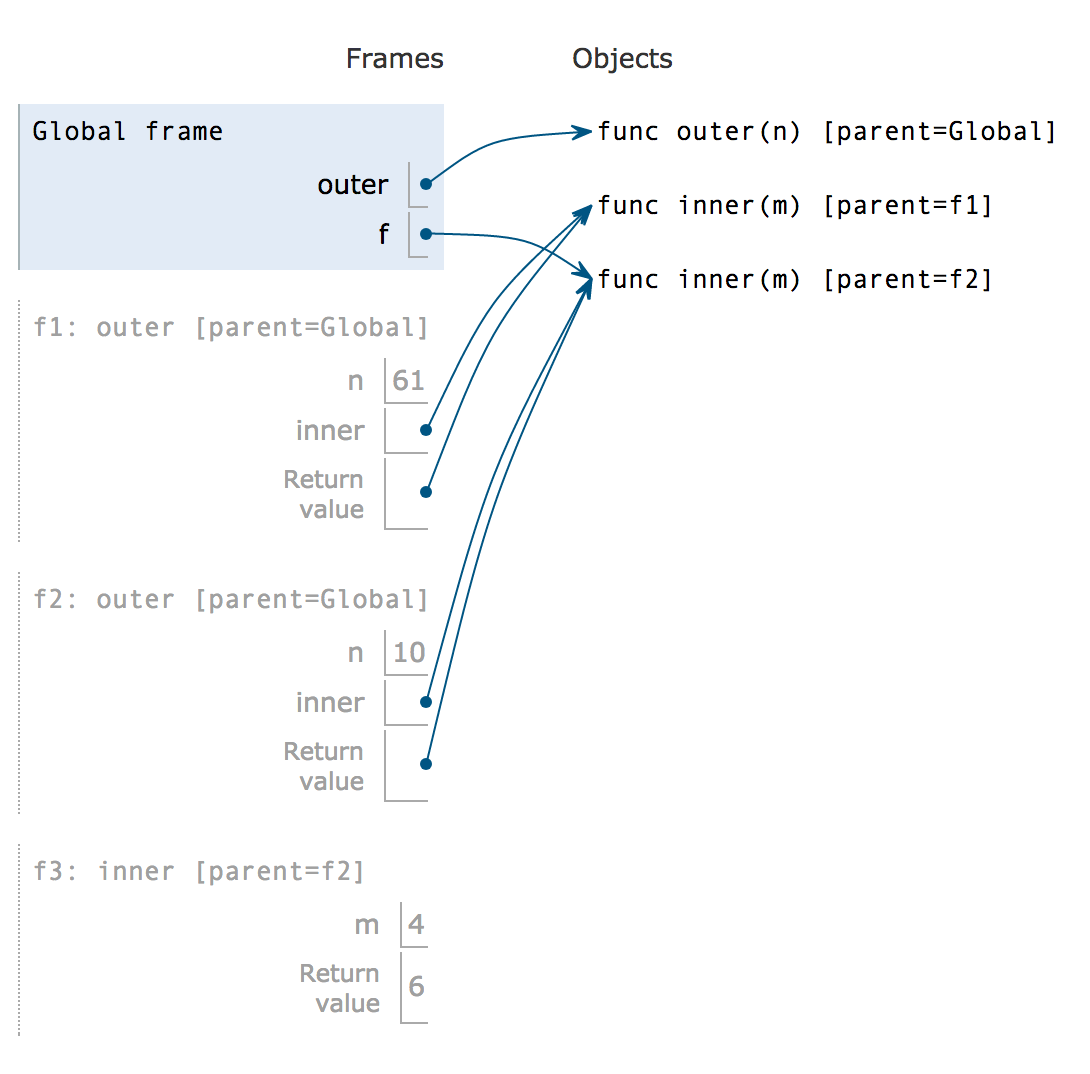
\includegraphics[width=300pt]{env-diagram.png} \\
Solution: https://goo.gl/pQmiEp \\
\href{https://www.youtube.com/watch?v=-7hkGrqM-4g&list=PLx38hZJ5RLZfg6jvEBBtjc5fnc5BclyEb&index=5}{Video Walkthrough}
\end{solution}

\question Using the same definition of \texttt{outer} above, what is the return
value of \texttt{outer(5)(4)}?

\begin{solution}[.2in]
\begin{lstlisting}
1
\end{lstlisting}
\end{solution}
\end{blocksection}
